% NOMAD Protocol - arXiv Preprint
% Network-Optimized Mobile Application Datagram
\documentclass[9pt,twocolumn]{article}

% Packages
\usepackage[utf8]{inputenc}
\usepackage[T1]{fontenc}
\usepackage{lmodern}
\usepackage{microtype}
\usepackage{graphicx}
\usepackage{booktabs}
\usepackage{tabularx}
\usepackage{amsmath}
\usepackage{amssymb}
\usepackage{hyperref}
\usepackage{cleveref}
\usepackage{listings}
\usepackage{xcolor}
\usepackage{balance}
\usepackage[margin=1in,columnsep=0.3in]{geometry}
\usepackage{fancyhdr}
\usepackage{caption}
\usepackage{subcaption}
\usepackage{tikz}
\usetikzlibrary{shapes,arrows,positioning,fit,backgrounds}

% Hyperref setup
\hypersetup{
    colorlinks=true,
    linkcolor=blue!70!black,
    citecolor=green!50!black,
    urlcolor=blue!70!black,
}

% Code listing style
\lstset{
    basicstyle=\ttfamily\small,
    breaklines=true,
    frame=single,
    numbers=left,
    numberstyle=\tiny\color{gray},
    keywordstyle=\color{blue!70!black},
    commentstyle=\color{green!50!black},
    stringstyle=\color{orange!70!black},
}

% Custom commands
\newcommand{\nomad}{\textsc{Nomad}}
\newcommand{\mosh}{\textsc{Mosh}}
\newcommand{\noise}{\textsc{Noise}}

% Title
\title{\textbf{NOMAD: A Secure State Synchronization Protocol\\for Mobile Applications over UDP}}

\author{
    Danyiel Colin\\
    \texttt{amaniel2718@protonmail.com}
}

\date{}

\begin{document}

\maketitle

% Abstract
\begin{abstract}
We present \nomad{} (Network-Optimized Mobile Application Datagram), a secure UDP-based state synchronization protocol for real-time applications over unreliable networks. Building on insights from \mosh{} (Mobile Shell), \nomad{} combines the \noise{} Protocol Framework's IK handshake pattern with XChaCha20-Poly1305 authenticated encryption to achieve mutual authentication in a single round-trip. The protocol features epoch-based rekeying for forward secrecy, seamless connection migration across IP address changes without reconnection, and an idempotent state synchronization layer that guarantees convergence despite packet loss and reordering. We formally verify the protocol's security properties using ProVerif and TLA+, discovering and fixing a post-compromise security vulnerability in the rekeying mechanism. A conformance test suite with over 1,000 test cases and a Rust reference implementation validate the design.
\end{abstract}

% Keywords
\noindent\textbf{Keywords:} UDP, state synchronization, Noise Protocol, authenticated encryption, mobile networking, roaming

\section{Introduction}
\label{sec:intro}

Remote shell access remains fundamental to system administration and software development. While SSH~\cite{rfc4253} provides secure connectivity, its TCP-based design leads to poor user experience over unreliable networks: connections freeze during packet loss, timeout during IP address changes, and require complete session reestablishment after network interruptions.

\mosh{} (Mobile Shell)~\cite{winstein2012mosh} addressed these limitations through a UDP-based State Synchronization Protocol (SSP), demonstrating that state synchronization with client-side prediction could achieve superior responsiveness. However, \mosh{}'s design is now over a decade old, and several aspects warrant modernization:

\begin{itemize}
    \item \textbf{Cryptographic primitives}: \mosh{} uses AES-128-OCB, while modern protocols favor ChaCha20-Poly1305 for software implementations
    \item \textbf{Key exchange}: \mosh{} bootstraps from SSH, whereas dedicated protocols like WireGuard~\cite{donenfeld2017wireguard} show the benefits of integrated key exchange
    \item \textbf{State generality}: \mosh{} is tightly coupled to terminal state, limiting reuse for other applications
\end{itemize}

We present \nomad{}, a new protocol that retains \mosh{}'s core insight---that idempotent state synchronization enables reliable operation over unreliable transport---while incorporating modern cryptographic practices and a generic state interface. \nomad{} is \emph{not} backward-compatible with \mosh{}, enabling a clean design unconstrained by legacy considerations.

\subsection{Contributions}

Our contributions are:

\begin{enumerate}
    \item A complete protocol specification across security, transport, and synchronization layers, using the \noise{} Protocol Framework~\cite{perrin2018noise} for 1-RTT mutual authentication

    \item An epoch-based rekeying mechanism providing forward secrecy with nonce namespace separation, preventing nonce reuse across key rotations

    \item Seamless connection migration where sessions survive IP address changes through cryptographic session identifiers, without requiring reconnection handshakes

    \item An idempotent state synchronization algorithm that guarantees convergence despite arbitrary packet loss and reordering

    \item A conformance test suite with over 1,000 test cases using property-based testing, test vectors generated from reference cryptographic libraries, and infrastructure for testing implementations in any language via Docker containers

    \item Formal verification using ProVerif and TLA+, including discovery and fix of a post-compromise security vulnerability in the rekeying mechanism
\end{enumerate}

\subsection{Paper Organization}

\Cref{sec:background} reviews relevant background on \mosh{}, the \noise{} Protocol Framework, and related work. \Cref{sec:design} presents the protocol design and layer architecture. \Cref{sec:security} details the security layer including handshake and rekeying. \Cref{sec:transport} describes the transport layer with roaming support. \Cref{sec:sync} explains the synchronization layer and convergence guarantees. \Cref{sec:extensions} covers the extension mechanism. \Cref{sec:evaluation} presents our conformance testing methodology. \Cref{sec:formal} describes formal verification results including a discovered vulnerability and fix. \Cref{sec:related} discusses related work, and \Cref{sec:conclusion} concludes.

\section{Background}
\label{sec:background}

\subsection{Mosh and State Synchronization}

\mosh{}~\cite{winstein2012mosh} introduced the State Synchronization Protocol (SSP) for remote terminal access. Its key insight is that for interactive applications, only the \emph{current} state matters---intermediate states can be skipped if the network is slow. This contrasts with TCP's reliable ordered delivery, which can cause unbounded buffering when bandwidth varies.

SSP maintains version numbers for local and remote state. Each frame carries a diff from a known base state to the current state. Because diffs are \emph{idempotent}---applying the same diff twice has no additional effect---duplicates and reorderings are harmless. The protocol simply always sends the diff from the last-acknowledged state to the current state.

\subsection{The Noise Protocol Framework}

The \noise{} Protocol Framework~\cite{perrin2018noise} provides a rigorous foundation for designing cryptographic handshake protocols. \noise{} defines handshake patterns specifying the sequence of Diffie-Hellman operations and when static keys are transmitted or known in advance.

\nomad{} uses the \texttt{Noise\_IK} pattern:
\begin{lstlisting}[frame=none,numbers=none]
Noise_IK(s, rs):
  <- s
  -> e, es, s, ss
  <- e, ee, se
\end{lstlisting}

In this pattern, the responder's static key (\texttt{s}) is known to the initiator beforehand (line 1). The initiator sends an ephemeral key and their encrypted static key (line 2), and the responder replies with an ephemeral key (line 3). The pattern provides mutual authentication in one round-trip, with identity hiding for the initiator.

\subsection{Authenticated Encryption}

\nomad{} uses XChaCha20-Poly1305~\cite{rfc8439} for authenticated encryption with associated data (AEAD). XChaCha20 extends ChaCha20's 12-byte nonce to 24 bytes, enabling random nonce generation without birthday-bound collision concerns. Poly1305 provides a 128-bit authentication tag.

\section{Protocol Design}
\label{sec:design}

\subsection{Design Goals}

\nomad{} targets the following goals:

\begin{enumerate}
    \item \textbf{Security}: End-to-end authenticated encryption with forward secrecy
    \item \textbf{Mobility}: Seamless operation across IP address changes
    \item \textbf{Latency}: Sub-100ms perceived latency via prediction
    \item \textbf{Simplicity}: Fixed cryptographic suite, no negotiation
    \item \textbf{Generality}: State-agnostic synchronization framework
\end{enumerate}

\subsection{Non-Goals}

To maintain simplicity, \nomad{} explicitly does not provide:
\begin{itemize}
    \item Backward compatibility with \mosh{}/SSP
    \item Cipher suite negotiation
    \item Reliable ordered delivery (applications handle via state sync)
    \item Multiplexing multiple state types per session
\end{itemize}

\subsection{Layer Architecture}

\nomad{} is organized into four layers, shown in \Cref{fig:layers}:

\begin{figure}[t]
\centering
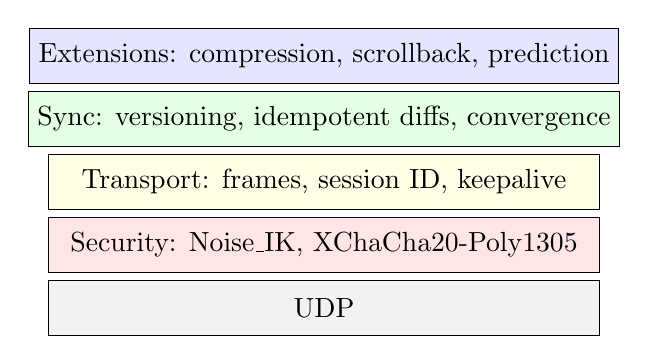
\begin{tikzpicture}[
    layer/.style={draw, rectangle, minimum width=7cm, minimum height=0.7cm, text centered},
    arrow/.style={->, thick}
]
    \node[layer, fill=blue!10] (ext) at (0,3) {Extensions: compression, scrollback, prediction};
    \node[layer, fill=green!10] (sync) at (0,2.2) {Sync: versioning, idempotent diffs, convergence};
    \node[layer, fill=yellow!10] (transport) at (0,1.4) {Transport: frames, session ID, keepalive};
    \node[layer, fill=red!10] (security) at (0,0.6) {Security: Noise\_IK, XChaCha20-Poly1305};
    \node[layer, fill=gray!10] (udp) at (0,-0.2) {UDP};
\end{tikzpicture}
\caption{NOMAD protocol layer stack.}
\label{fig:layers}
\end{figure}

\begin{description}
    \item[Security Layer] Handles the \noise{} IK handshake, AEAD encryption, and periodic rekeying for forward secrecy.

    \item[Transport Layer] Manages frame construction, session identification via 48-bit session IDs, connection migration (roaming), RTT estimation, and keepalive.

    \item[Sync Layer] Implements versioned state synchronization with idempotent diffs and acknowledgment tracking.

    \item[Extensions] Optional features negotiated during handshake: compression, scrollback, and client-side prediction.
\end{description}

\subsection{Cryptographic Suite}

\nomad{} uses a \emph{fixed} cryptographic suite with no runtime negotiation:

\begin{table}[h]
\centering
\begin{tabular}{ll}
\toprule
\textbf{Purpose} & \textbf{Algorithm} \\
\midrule
Key Exchange & X25519 \\
AEAD Cipher & XChaCha20-Poly1305 \\
Hash Function & BLAKE2s-256 \\
Key Derivation & HKDF-BLAKE2s \\
\bottomrule
\end{tabular}
\caption{Fixed cryptographic suite.}
\label{tab:crypto}
\end{table}

If vulnerabilities are discovered, a new protocol version is released rather than negotiating alternatives. This follows WireGuard's philosophy of ``cryptographic versioning.''

\section{Security Layer}
\label{sec:security}

\subsection{Handshake Protocol}

The handshake establishes a session between initiator and responder in one round-trip. The initiator must know the responder's static public key beforehand (obtained via SSH, QR code, or other secure channel).

\subsubsection{Handshake Initiation}

The initiator sends:
\begin{itemize}
    \item Protocol version (2 bytes)
    \item Ephemeral public key (32 bytes, unencrypted)
    \item Static public key (32 bytes + 16 byte tag, encrypted)
    \item Payload with state type ID and extensions (encrypted)
\end{itemize}

The initiator's static key is encrypted after the first DH operation, providing identity hiding from passive observers.

\subsubsection{Handshake Response}

The responder replies with:
\begin{itemize}
    \item Session ID (6 bytes)
    \item Ephemeral public key (32 bytes, unencrypted)
    \item Acknowledgment and negotiated extensions (encrypted)
\end{itemize}

After successful handshake, both parties derive symmetric session keys using HKDF with the handshake transcript hash.

\subsection{Session Keys}

Session keys are derived as:
\begin{equation}
(k_i, k_r) = \text{HKDF}(h, \text{``nomad v1 keys''}, 64)
\end{equation}
where $k_i$ and $k_r$ are the initiator and responder keys, and $h$ is the handshake hash.

The initiator uses $k_i$ for sending and $k_r$ for receiving; the responder uses the inverse.

\subsection{Nonce Construction}

XChaCha20-Poly1305 requires 24-byte nonces. \nomad{} constructs nonces as:

\begin{table}[h]
\centering
\begin{tabular}{lll}
\toprule
\textbf{Field} & \textbf{Size} & \textbf{Description} \\
\midrule
Epoch & 4 bytes & Current epoch number \\
Direction & 1 byte & 0x00 or 0x01 \\
Zeros & 11 bytes & Padding \\
Counter & 8 bytes & Per-direction counter \\
\bottomrule
\end{tabular}
\caption{Nonce structure (24 bytes total).}
\end{table}

The epoch field provides nonce namespace separation across rekeying operations, ensuring nonce uniqueness even as counters reset.

\subsection{Rekeying}

Sessions rekey periodically for forward secrecy. \Cref{tab:rekey} shows the timing constants.

\begin{table}[h]
\centering
\begin{tabular}{ll}
\toprule
\textbf{Constant} & \textbf{Value} \\
\midrule
\texttt{REKEY\_AFTER\_TIME} & 120 seconds \\
\texttt{REJECT\_AFTER\_TIME} & 180 seconds \\
\texttt{REKEY\_AFTER\_MESSAGES} & $2^{60}$ \\
\texttt{REJECT\_AFTER\_MESSAGES} & $2^{64}-1$ \\
\texttt{OLD\_KEY\_RETENTION} & 5 seconds \\
\bottomrule
\end{tabular}
\caption{Rekeying timing constants.}
\label{tab:rekey}
\end{table}

During rekeying, both parties perform a fresh ephemeral DH exchange. After key rotation, nonce counters reset to zero and the epoch increments. Old keys are retained briefly (5 seconds) to decrypt in-flight packets, then securely zeroed.

\subsection{Anti-Replay Protection}

Each endpoint maintains a sliding window of at least 2048 received nonce values. The replay check occurs \emph{before} AEAD verification to prevent CPU exhaustion attacks via replayed packets forcing expensive decryption operations.

\subsection{Security Properties}

\Cref{tab:security} summarizes the security properties provided.

\begin{table}[h]
\centering
\begin{tabular}{ll}
\toprule
\textbf{Property} & \textbf{Mechanism} \\
\midrule
Confidentiality & XChaCha20-Poly1305 \\
Integrity & Poly1305 tag \\
Authenticity & Noise\_IK mutual auth \\
Forward secrecy & Ephemeral DH + rekeying \\
Replay protection & Nonce window \\
Initiator identity hiding & Encrypted static key \\
\bottomrule
\end{tabular}
\caption{Security properties.}
\label{tab:security}
\end{table}

\section{Transport Layer}
\label{sec:transport}

\subsection{Frame Format}

Data frames carry encrypted sync messages:

\begin{table}[h]
\centering
\begin{tabular}{lll}
\toprule
\textbf{Field} & \textbf{Size} & \textbf{Encrypted} \\
\midrule
Type & 1 byte & No \\
Flags & 1 byte & No \\
Session ID & 6 bytes & No \\
Nonce Counter & 8 bytes & No \\
Payload & variable & Yes \\
AEAD Tag & 16 bytes & N/A \\
\bottomrule
\end{tabular}
\caption{Data frame format.}
\end{table}

The 16-byte header (type through nonce counter) serves as additional authenticated data (AAD) for AEAD, preventing header tampering.

\subsection{Connection Migration (Roaming)}

\nomad{} supports seamless IP address migration. When an authenticated frame arrives from a new source address:

\begin{enumerate}
    \item Verify the AEAD tag with current session keys
    \item If valid: update the remote endpoint to the new address
    \item If invalid: silently drop (prevents spoofing)
\end{enumerate}

No handshake is required. The session ID cryptographically binds the connection across IP changes. Anti-amplification limits (3$\times$ received bytes) prevent DDoS abuse.

\subsection{RTT Estimation}

Each frame carries timestamps for RTT measurement:
\begin{itemize}
    \item \textbf{Timestamp}: Sender's time since session start (ms)
    \item \textbf{Timestamp Echo}: Most recent timestamp received from peer
\end{itemize}

RTT samples update smoothed RTT (SRTT) and variance using the RFC 6298 algorithm. The retransmission timeout (RTO) adapts accordingly, bounded between 100ms and 60 seconds.

\subsection{Frame Pacing}

To prevent congestion, frame transmission is paced:

\begin{table}[h]
\centering
\begin{tabular}{ll}
\toprule
\textbf{Constant} & \textbf{Value} \\
\midrule
\texttt{MIN\_FRAME\_INTERVAL} & max(SRTT/2, 20ms) \\
\texttt{COLLECTION\_INTERVAL} & 8ms \\
\texttt{DELAYED\_ACK\_TIMEOUT} & 100ms \\
\texttt{MAX\_FRAME\_RATE} & 50 Hz \\
\bottomrule
\end{tabular}
\caption{Frame pacing constants.}
\end{table}

The collection interval batches rapid state changes (e.g., fast typing) into single frames. Delayed acknowledgment allows acks to piggyback on data frames.

\section{Synchronization Layer}
\label{sec:sync}

\subsection{State Interface}

Any state type implementing the following interface can be synchronized:

\begin{lstlisting}[language=Python]
class SyncState(Protocol):
    STATE_TYPE_ID: str  # e.g., "nomad.terminal.v1"

    def diff(self, old: Self, new: Self) -> bytes:
        """Create idempotent diff."""

    def apply(self, state: Self, diff: bytes) -> Self:
        """Apply diff (must be idempotent)."""
\end{lstlisting}

The critical requirement is that diffs be \emph{idempotent}: applying the same diff twice has no additional effect. This enables correct operation despite duplicates and reordering.

\subsection{Sync Message Format}

\begin{table}[h]
\centering
\begin{tabular}{ll}
\toprule
\textbf{Field} & \textbf{Size} \\
\midrule
Sender State Number & 8 bytes \\
Acked State Number & 8 bytes \\
Base State Number & 8 bytes \\
Diff Length & 4 bytes \\
Diff Payload & variable \\
\bottomrule
\end{tabular}
\caption{Sync message format.}
\end{table}

\subsection{Convergence Algorithm}

The receiver applies diffs based on version comparison:

\begin{lstlisting}[language=Python]
def receive_sync(msg):
    # Update ack tracking
    if msg.acked > last_acked:
        last_acked = msg.acked

    # Apply if newer (idempotent)
    if msg.sender_state_num > peer_state_num:
        peer_state = apply(peer_state, msg.diff)
        peer_state_num = msg.sender_state_num
\end{lstlisting}

The algorithm guarantees eventual consistency: regardless of packet loss, reordering, or duplication, states converge when any message gets through.

\subsection{State Skipping}

A consequence of state synchronization is that intermediate states may be lost if the network is slow. For terminal applications, this means fast output scrolls past without buffering. This is acceptable for interactive use but applications needing full history should use different transports.

\section{Extensions}
\label{sec:extensions}

Extensions use Type-Length-Value (TLV) encoding and are negotiated during handshake. Defined extensions:

\begin{description}
    \item[Compression (0x0001)] zstd compression of diff payloads with configurable level (1--22). Small payloads may skip compression if it would increase size.

    \item[Scrollback (0x0002)] Terminal-specific: synchronizes scrollback buffer for accessing previous output.

    \item[Prediction (0x0003)] Terminal-specific: enables client-side keystroke prediction for perceived sub-10ms latency.
\end{description}

Future extensions include multiplexing and post-quantum key exchange (hybrid X25519+ML-KEM).

\section{Evaluation}
\label{sec:evaluation}

\subsection{Conformance Test Suite}

We developed a conformance test suite to validate protocol implementations. The suite is organized into phases:

\begin{description}
    \item[Phase 1 (No Docker)] Validates a Python reference codec against generated test vectors. Tests cover cryptographic primitives, handshake logic, and sync message encoding.

    \item[Phase 2 (Docker)] Tests real implementations via containerization, including wire format compliance, adversarial inputs, and network resilience.
\end{description}

\subsection{Test Categories}

\begin{table}[h]
\centering
\begin{tabular}{lrr}
\toprule
\textbf{Category} & \textbf{Tests} & \textbf{Docker} \\
\midrule
Unit (reference codec) & 80 & No \\
Protocol (handshake, rekey) & 107 & No \\
Adversarial (replay, MITM) & 36 & No \\
Resilience (packet loss, jitter) & 60+ & Yes \\
Wire (byte-level format) & 40+ & Yes \\
\midrule
\textbf{Total} & \textbf{1,000+} & \\
\bottomrule
\end{tabular}
\caption{Test suite coverage.}
\end{table}

\subsection{Test Vector Generation}

Test vectors are generated using reference cryptographic libraries (Python \texttt{cryptography} for XChaCha20-Poly1305, \texttt{noiseprotocol} for Noise\_IK). Generation is idempotent---running twice produces identical output---ensuring reproducibility. Vectors are stored in JSON5 format with inline comments explaining each field.

\subsection{Property-Based Testing}

We use Hypothesis~\cite{hypothesis} for property-based testing. Key properties verified:
\begin{itemize}
    \item Idempotence: $a(s,d) = a(a(s,d), d)$ where $a$ is apply
    \item Convergence: arbitrary orderings reach same state
    \item Replay rejection: repeated nonces detected
    \item Nonce uniqueness: no collisions within epoch
\end{itemize}

\subsection{Reference Implementation}

A Rust implementation of \nomad{} (\texttt{nomad-protocol} crate) has passed the complete conformance suite including all unit, protocol, and adversarial tests. The implementation is available on crates.io.

\section{Formal Verification}
\label{sec:formal}

We formally verify \nomad{}'s security properties using ProVerif~\cite{blanchet2016proverif} for cryptographic protocol analysis and TLA+~\cite{lamport2002tla} for state machine verification.

\subsection{ProVerif Security Analysis}

We model the handshake, replay protection, and rekeying mechanisms in ProVerif's applied pi-calculus. \Cref{tab:proverif} summarizes the verified properties.

\begin{table}[h]
\centering
\begin{tabular}{ll}
\toprule
\textbf{Property} & \textbf{Result} \\
\midrule
Session key secrecy & Verified \\
Mutual authentication & Verified \\
Frame authenticity & Verified \\
Replay protection & Verified \\
Forward secrecy & Verified \\
Post-compromise security & Verified* \\
\bottomrule
\end{tabular}
\caption{ProVerif verification results. *After fix.}
\label{tab:proverif}
\end{table}

\subsubsection{PCS Vulnerability Discovery and Fix}

ProVerif identified a vulnerability in the original rekeying mechanism: an attacker who compromises epoch $n$ session keys can perform a man-in-the-middle attack during the epoch $n+1$ rekey, maintaining access indefinitely.

The attack exploits that rekey messages were authenticated only with the current (compromised) session key. The attacker intercepts the initiator's new ephemeral key, generates their own ephemeral, and completes the rekey with both parties---deriving the new session keys.

We fix this by deriving a \texttt{rekey\_auth\_key} from the static Diffie-Hellman secret during handshake:
\begin{equation}
k_{auth} = \text{HKDF}(\text{DH}(s_i, S_r), \text{``rekey auth''})
\end{equation}

New session keys mix this authentication key:
\begin{equation}
(k'_i, k'_r) = \text{HKDF}(\text{DH}(e_i, e_r) \| k_{auth}, n)
\end{equation}

Since the attacker lacks the static private keys, they cannot compute $k_{auth}$ and thus cannot derive valid epoch $n+1$ keys. ProVerif confirms this fix restores post-compromise security.

\subsection{TLA+ State Machine Verification}

We model three protocol components in TLA+ and verify safety invariants using the TLC model checker. \Cref{tab:tlaplus} shows the verification results.

\begin{table}[h]
\centering
\begin{tabular}{lrr}
\toprule
\textbf{Model} & \textbf{States} & \textbf{Invariants} \\
\midrule
Rekey state machine & 2.8M & 6 \\
Sync layer & 200K & 6 \\
Roaming & 41K & 6 \\
\bottomrule
\end{tabular}
\caption{TLA+ model checking results.}
\label{tab:tlaplus}
\end{table}

Key invariants verified include: monotonic epoch numbers, nonce uniqueness within epochs, anti-amplification bounds during roaming, and eventual state convergence (given bounded message loss).

The formal models are available in the \texttt{formal/} directory of the specification repository.

\section{Related Work}
\label{sec:related}

\Cref{tab:comparison} compares \nomad{} with related protocols.

\begin{table*}[t]
\centering
\begin{tabular}{lllll}
\toprule
\textbf{Property} & \textbf{NOMAD} & \textbf{Mosh} & \textbf{WireGuard} & \textbf{QUIC} \\
\midrule
Transport & UDP & UDP & UDP & UDP \\
Handshake RTT & 1 & 0 (SSH bootstrap) & 1 & 1--2 \\
AEAD & XChaCha20-Poly1305 & AES-128-OCB & ChaCha20-Poly1305 & AES-GCM/ChaCha20 \\
Key Exchange & Noise\_IK & N/A (SSH) & Noise\_IK & TLS 1.3 \\
Roaming & Yes & Yes & Yes & Yes (CID) \\
Forward Secrecy & Yes (2 min rekey) & No & Yes (2 min rekey) & Yes \\
State Sync & Yes & Yes & No & No \\
Cipher Negotiation & No & No & No & Yes \\
\bottomrule
\end{tabular}
\caption{Protocol comparison.}
\label{tab:comparison}
\end{table*}

\textbf{Mosh}~\cite{winstein2012mosh} pioneered UDP-based state synchronization for remote shells. \nomad{} inherits its core insight but updates the cryptographic primitives and adds forward secrecy via rekeying.

\textbf{WireGuard}~\cite{donenfeld2017wireguard} demonstrated that fixed cryptographic suites and minimal code simplify security analysis. \nomad{} follows this philosophy and borrows WireGuard's rekeying approach.

\textbf{QUIC}~\cite{rfc9000} provides reliable transport over UDP with integrated TLS 1.3. Unlike \nomad{}, QUIC provides ordered delivery and requires more complex connection state.

\textbf{SSH}~\cite{rfc4253} remains the standard for secure remote access but suffers from TCP's limitations on unreliable networks.

\section{Conclusion}
\label{sec:conclusion}

We presented \nomad{}, a secure state synchronization protocol combining modern cryptography with the proven SSP paradigm from \mosh{}. The protocol achieves mutual authentication in one RTT using the Noise\_IK pattern, provides forward secrecy through periodic rekeying, supports seamless roaming across IP changes, and guarantees state convergence through idempotent diffs.

Our conformance test suite with over 1,000 tests and property-based verification provides confidence in implementation correctness. The layered design separates concerns cleanly, and the generic state interface enables applications beyond terminal emulation.

Future work includes formal verification of the security properties, performance benchmarking under various network conditions, and development of additional state types for collaborative applications.

\subsection*{Availability}

The protocol specifications and conformance test suite are available as open source. The Rust reference implementation is published at \url{https://crates.io/crates/nomad-protocol}.

% Balance columns on last page
\balance

\bibliographystyle{plain}
\bibliography{references}

\end{document}
